\documentclass[11pt]{article}
\usepackage[margin=0.72in]{geometry}
\usepackage{times}
\usepackage{booktabs}
\usepackage{graphicx}
\usepackage{amsmath}
\usepackage{microtype}
\usepackage{enumitem}
\usepackage{caption}
\usepackage{hyperref}
\usepackage[T1]{fontenc}
\usepackage[utf8]{inputenc}
\setlist{nosep,leftmargin=1.2em}
\captionsetup{font=small,skip=3pt}
\hypersetup{colorlinks=true,linkcolor=black,citecolor=black,urlcolor=blue}
\pagestyle{plain}
\setlength{\parskip}{0.28em}
\setlength{\parindent}{0pt}

\title{\vspace{-1.6em}Assignment 1: Fine-Tune, Sanitize, Extract\\[0.2em]
\large COL873 / ELL8299 --- Trustworthy Large Language Models}
\author{Abhiram Dharme \quad (cs5221139)\\
Indian Institute of Technology Delhi}
\date{Semester I, 2026--27}

\begin{document}
\maketitle
\vspace{-1.5em}

\begin{abstract}
\noindent
We adapt Qwen2.5-1.5B-Instruct with LoRA as a PII sanitizer on the frozen ai4privacy split, then sanitize a victim corpus and attack Qwen2.5-0.5B. Adapter \emph{placement} (not rank) buys most of the F1; A2 (full attention, $r{=}8$) is selected for lowest validation leak. On in-distribution test, A2 reaches exact entity F1 $0.922$ and leak $0.031$, beating regex, Presidio, and zero-shot. Near-OOD F1 collapses to $0.178$ from a label-set shift. Sanitizing the victim corpus raises held-out PPL from $9.41$ to $14.78$ (pretrained $14.25$) while cutting untargeted PII recovery $1031{\to}194$ and targeted member leak $0.41{\to}0.02$. Canary secrets are rewritten as \texttt{[PASSPORT]}; residual extraction is list-position email misses, not the Secret-Sharer template.
\end{abstract}

\vspace{-0.45em}
\section{Setup}
\vspace{-0.15em}
All rows come from the supplied bundle; \texttt{data/manifest.jsonl} is verified before training. Loss is completion-only: chat-template prompt tokens are labelled $-100$. Effective batch 16, seed 42, 2 epochs (sanitizer) / 4 epochs (victims), cosine LR $2{\times}10^{-4}$ with 3\% warmup, LoRA dropout 0.05. Runs used IITD HPC \texttt{scai\_q} (A100 80\,GB, bf16, microbatch 16). Trainable counts are from PEFT; peak memory from \texttt{cuda.max\_memory\_allocated}. A6 is the 4-bit exception.

\section{Part A --- Where the adapters go}
\vspace{-0.15em}
\paragraph{Selection rule.}
Lowest validation leak, then highest exact entity F1, then fewer trainable parameters. Leak is the fraction of gold PII values that still appear verbatim in the generation (case-insensitive, whitespace-normalized). Entity F1 is exact span+label match after span recovery (Section~\ref{sec:b}).

\begin{table}[t]
\centering
\caption{Part~A validation sweep (A100, seed 42, 2 epochs). A2 is leak-first; A4 is the F1 peak.}
\label{tab:sweep}
\scriptsize
\setlength{\tabcolsep}{3.0pt}
\begin{tabular}{@{}l l r r r r r r r@{}}
\toprule
ID & Modules & $r$ & $\alpha$ & Trainable & Peak GB & Wall (s) & F1 & Leak \\
\midrule
A1 & $q,v$ & 8 & 16 & 1.09M (0.071\%) & 50.57 & 1361 & 0.897 & 0.0306 \\
A2 & attn & 8 & 16 & 2.18M (0.141\%) & 53.44 & 1461 & 0.917 & \textbf{0.0274} \\
A3 & attn+MLP & 8 & 16 & 9.23M (0.595\%) & 64.67 & 1932 & 0.940 & 0.0291 \\
A4 & attn+MLP & 32 & 64 & 36.9M (2.34\%) & 65.20 & 1948 & \textbf{0.945} & 0.0291 \\
A5 & attn+MLP & 32 & 16 & 36.9M (2.34\%) & 65.20 & 1943 & 0.937 & 0.0292 \\
A6 & attn+MLP 4b & 32 & 64 & 36.9M (3.99\%) & 24.43 & 3496 & 0.934 & 0.0305 \\
\bottomrule
\end{tabular}
\end{table}

\begin{figure}[t]
\centering
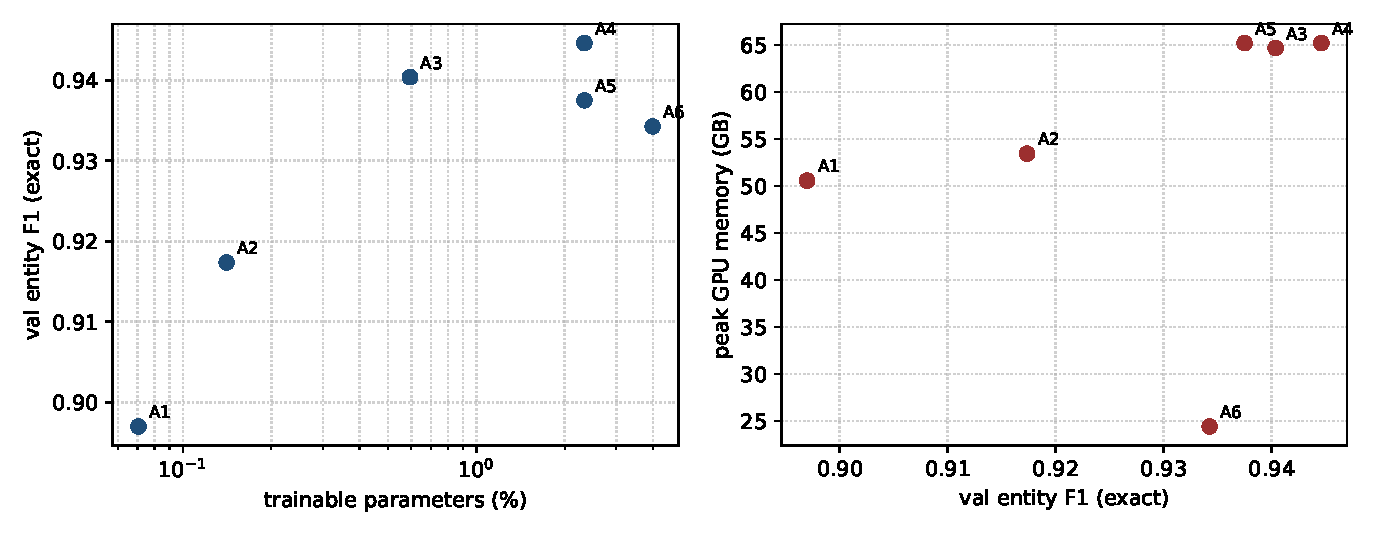
\includegraphics[width=\textwidth]{figures/partA_fig.pdf}
\caption{Left: exact val F1 vs.\ trainable percentage (log $x$). Right: peak GPU memory vs.\ F1. Placement (A1$\to$A3) moves the curve; rank (A3$\to$A5) does not. A6 is the memory outlier.}
\label{fig:sweep}
\end{figure}

\paragraph{Placement vs.\ rank vs.\ $\alpha$.}
A1$\to$A2 (add $k,o$) costs $+1.09$M parameters and $+100$\,s for $+2.0$ F1 points and the best leak. A2$\to$A3 (add MLP) is the remaining F1 step ($+2.3$ points) at $4.2{\times}$ trainable weights, $+11$\,GB, and $+8$ minutes; leak rises slightly. A3$\to$A5 ($r{:}8\to 32$, $\alpha$ fixed) is a dead axis: F1 drops $0.3$ points at $4{\times}$ rank. A5$\to$A4 ($\alpha{:}16\to 64$) recovers a little F1 ($0.937\to 0.945$) at identical memory and wall-clock. F1-per-parameter ranking is A1 $\gg$ A2 $\gg$ A3 $\gg$ A4/A5; the curve flattens once MLP is adapted.

\paragraph{QLoRA.}
A6 matches A4 on a 4-bit base. Peak memory falls from 65.2\,GB to 24.4\,GB ($\sim$2.7$\times$). Wall-clock goes the other way: 3496\,s vs 1948\,s (0.72 vs 1.28 it/s). F1 0.934 vs 0.945; leak 0.0305 vs 0.0291. QLoRA cost a little accuracy and did not save time; it did save memory.

\paragraph{Choice.}
A4 is the F1 peak; A2 is the leak minimum with less than a quarter of A4's trainable mass. We copy A2 as \texttt{best\_sanitizer} for Parts~B and~C.

\section{Part B --- Sanitizer evaluation}
\label{sec:b}
\vspace{-0.15em}
The model emits masked text, not offsets. We recover $(\mathrm{start},\mathrm{end},\mathrm{label})$ by a literal-gap walk: split the prediction on \texttt{[LABEL]} placeholders, locate each literal left-to-right in the source, and treat the intervening source substring as the predicted span (split when several placeholders share one gap). If a literal cannot be found, \texttt{difflib.SequenceMatcher} maps replaced source regions onto placeholders. Counted failure modes: several placeholders collapsing onto one name, a placeholder with no residual source, coarse opcode spans, and OOD label-set shift (\texttt{GIVENNAME1} vs.\ \texttt{FIRSTNAME}).

\begin{table}[t]
\centering
\caption{In-distribution test ($n{=}2000$) and near-OOD ($n{=}1000$). Exact = span+label; IoU = overlap ${\ge}0.5$+label. FT is A2.}
\label{tab:b}
\scriptsize
\setlength{\tabcolsep}{2.4pt}
\begin{tabular}{@{}l r r r r r r r@{}}
\toprule
System & Exact F1 & Macro & IoU F1 & Leak & Over-mask & Well-formed \\
\midrule
FT (A2) & \textbf{0.922} & \textbf{0.900} & \textbf{0.927} & \textbf{0.031} & 0.010 & \textbf{0.993} \\
Regex & 0.385 & 0.301 & 0.423 & 0.426 & 0.009 & 0.978 \\
Presidio & 0.256 & 0.157 & 0.277 & 0.421 & 0.019 & 0.983 \\
Zero-shot & 0.108 & 0.092 & 0.118 & 0.674 & 0.112 & 0.895 \\
\midrule
FT OOD & 0.178 & 0.125 & 0.196 & 0.297 & 0.003 & 0.236 \\
Regex OOD & 0.191 & 0.090 & 0.216 & 0.764 & 0.003 & 0.880 \\
Presidio OOD & 0.198 & 0.090 & 0.218 & 0.434 & 0.013 & 0.835 \\
\bottomrule
\end{tabular}
\end{table}

\begin{table}[t]
\centering
\caption{A2 per-class exact F1 on the 10 most frequent ID labels (support in parentheses).}
\label{tab:perclass}
\scriptsize
\setlength{\tabcolsep}{3.2pt}
\begin{tabular}{@{}l r l r@{}}
\toprule
Label & F1 ($n$) & Label & F1 ($n$) \\
\midrule
TIME & 0.930 (945) & DRIVERLICENSE & 0.898 (643) \\
USERNAME & 0.940 (760) & LASTNAME1 & 0.844 (623) \\
SOCIALNUMBER & 0.957 (668) & BOD & 0.958 (553) \\
EMAIL & 0.975 (662) & PASSPORT & 0.863 (552) \\
IDCARD & 0.893 (651) & SEX & 0.949 (529) \\
\bottomrule
\end{tabular}
\end{table}

\paragraph{Baselines.}
Regex is field-aware (email, phone, IP, card, date/time, URL, SSN/passport/IDs, labelled \texttt{key: value} extractors). Presidio uses default recognizers with spaCy \texttt{en\_core\_web\_sm}. Zero-shot is the same 1.5B instruct model with no adapter. Fine-tuning is the entire gain: leak drops $0.426{\to}0.031$ vs regex; F1 more than doubles.

\paragraph{OOD.}
The OOD file uses \texttt{FIRSTNAME}, \texttt{LASTNAME}, \texttt{PREFIX} rather than \texttt{GIVENNAME1}/\texttt{LASTNAME1}. A2 still emits the 300k inventory, so exact F1 is 0.178 and well-formedness 0.236: most predictions are ``wrong'' by label identity even when a name was redacted. Leak 0.297 is still below regex (0.764). This is a schema shift, not a claim of real-world coverage.

\paragraph{Error taxonomy (ID leaks, 463 gold values).}
Not uniform across classes. \texttt{SEX}: 135/529 (26\%) --- tokens such as \texttt{Male}/\texttt{Female} remain as ordinary English after a nearby \texttt{[SEX]} is emitted. \texttt{STATE}: 124/513 (24\%) --- two-letter codes (\texttt{IN}, \texttt{OR}) collide with English words. \texttt{COUNTRY}: 68/384 (18\%). Structured identifiers are rare: \texttt{EMAIL} 5, \texttt{TEL} 6, \texttt{IDCARD} 4. Remaining leaks are short, high-frequency strings, not missed SSNs.

\section{Part C --- Extraction attacks}
\vspace{-0.15em}
Two victims share PEFT ($r{=}32$, $\alpha{=}64$, all attn+MLP, 4 epochs, seed 42) on Qwen2.5-0.5B: V-raw on the supplied corpus; V-san on the same 8{,}007 rows after A2, metadata preserved, canaries not exempted. Victim PEFT is held fixed, as C.2 requires; the privacy change below is the corpus, not adapter placement. Held-out PPL on \texttt{partC\_heldout.jsonl} is the utility axis. Attacks run on V-raw, V-san, and the untuned base.

\begin{table}[t]
\centering
\caption{Part~C: utility vs.\ extraction. $P{*}{=}100$ is the best of the four membership scores. Exposure is mean sampled-rank bits at $n_{\mathrm{reps}}{=}64$.}
\label{tab:c}
\scriptsize
\setlength{\tabcolsep}{2.6pt}
\begin{tabular}{@{}l r r r r r r r@{}}
\toprule
Model & PPL & Disc.\ all & $n{=}32$ & $P{*}{=}100$ & PII str. & Exp$_{64}$ & Tgt top-1 \\
\midrule
V-raw & 9.41 & 3.4\% & 100\% & 0.85 & 1031 & 13.29 & 0.41 \\
V-san & 14.78 & 1.9\% & 18\% & 0.04 & 194 & 2.33 & 0.02 \\
Pretrained & 14.25 & 0.02\% & 0\% & 0.00 & 12 & 3.12 & 0.01 \\
\bottomrule
\end{tabular}
\end{table}

Discoverable exact-match by $n_{\mathrm{reps}}$ on V-raw is 0.6\% ($n{=}1$), 12\% ($n{=}2$), 97\% ($n{=}8$), 100\% ($n{=}32$). V-san stays $\sim$18--21\% even at $n{=}8,32$: the model memorizes placeholder-regularized suffixes, not the original PII. Untargeted: 5{,}000 samples ranked by $\mathrm{ppl}$, $\mathrm{ratio_{ref}}$, $\mathrm{ratio_{lower}}$, $\mathrm{ratio_{zlib}}$; V-raw $P{*}{=}100 \in [0.80,0.85]$ with 20 distinct training docs; V-san $0.02$--$0.04$. Targeted (200 member / 200 control): V-raw greedy/sampled member leak $0.41$/$0.445$ vs control $0.045$/$0.09$; V-san $0.02$/$0.015$ vs $0.03$/$0.055$ (no membership gap). Utility cost is essentially ``return to pretrained PPL'' ($+5.37$).

\begin{figure}[t]
\centering
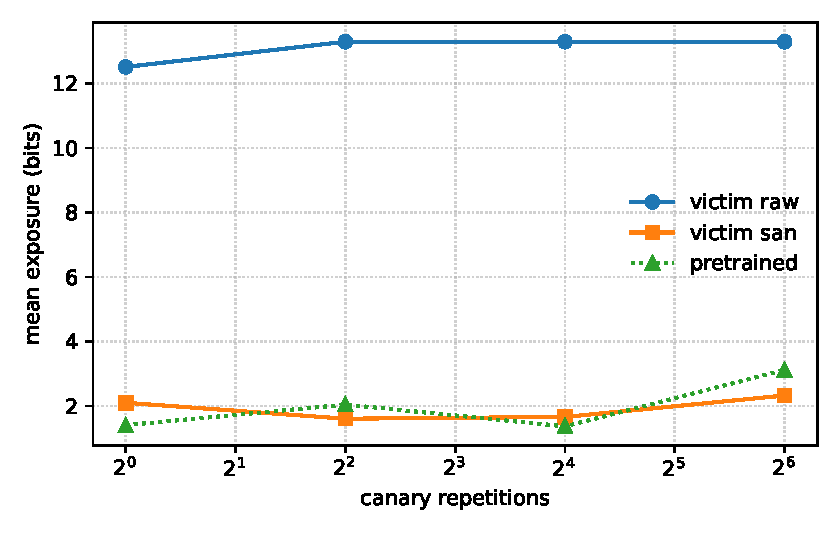
\includegraphics[width=0.82\textwidth]{figures/partC_exposure.pdf}
\caption{Mean canary exposure vs.\ repetition. V-raw saturates the sampled-rank ceiling; V-san tracks the pretrained control.}
\label{fig:exp}
\end{figure}

\paragraph{Canary exposure.}
True six-digit secrets ranked against 9{,}999 alternatives; $\mathrm{exposure}\approx \log_2 10^6 - \log_2\hat{r}$ with $\hat{r}=(\mathrm{rank_{sample}}/10^4)\times 10^6$. Rank-1 in the sample implies $\hat{r}{=}100$ and $\approx 13.29$ bits, not $\log_2 10^6\approx 19.9$. That ceiling is the estimator. V-raw hits it for every canary with $n_{\mathrm{reps}}\ge 4$. A2 rewrote every canary as \texttt{[PASSPORT]} (0/425 canary rows still contain the secret), so V-san exposure ($1.6$--$2.3$ bits) matches pretrained.

\paragraph{Two traced leaks (redacted).}
Canaries were not the failure. (1)~List-position miss: in a numbered patient block, items 1--12 become \texttt{[EMAIL]} while item 13 keeps \texttt{ra***@gmail.com}. (2)~Truncated local-part: a comma list is emitted as \texttt{9***@yahoo.com, [EMAIL], [EMAIL], [EMAIL]} --- the first address is shortened and left literal. 36 sanitized corpus rows still contain an email regex; those leftovers, not the Secret-Sharer template, are the plausible source of V-san's residual 194 verified PII strings.

\section{What we would do next}
\vspace{-0.15em}
A2 still leaks $\sim$3\% of gold values, concentrated in short closed-class tokens, and MLP adapters raised F1 without lowering leak. Next defenses, in order of F1-per-hour: (1)~a second pass that redacts any remaining string matching the training PII lexicon (membership over values, not generation) --- this would have caught the leftover emails; (2)~forbid emitting a gold SEX/STATE/COUNTRY token that still occurs as a whole word; (3)~goldfish / token-dropping~\cite{hans2024goldfish} or DP-SGD LoRA~\cite{yu2022dplm} on residual-risk canaries rather than the 1.5B sanitizer. Reject any candidate that increases leak on a held-out canary split even if F1 rises.

\section*{Honour code}
\vspace{-0.15em}
{\small Even though I have taken help from the following students and LLMs in terms of discussing ideas and coding practices, all my code is written by me.}

Students consulted: None.

LLMs/tools: a coding assistant for boilerplate, environment wiring, and debugging. Training, metrics, and numbers are from the HPC A100 run described above.

\appendix
\section{Hyperparameters and prompt}
\vspace{-0.1em}
Sanitizer: Qwen2.5-1.5B-Instruct, AdamW, cosine, warmup 0.03, grad clip 1.0, max length 768. Victim: Qwen2.5-0.5B base (not instruct), max length 512. System prompt (abbreviated): copy the user text, replace every private value by \texttt{[LABEL]} from the 300k label set, keep all other characters, output only the sanitized text. Span recovery: \texttt{src/lib/align.py}. Every number is reproducible from \texttt{run\_all.sh} with seed 42.

\begin{thebibliography}{9}
\bibitem{hu2022lora}
E.~Hu et al., ``LoRA,'' ICLR, 2022.
\bibitem{dettmers2023qlora}
T.~Dettmers et al., ``QLoRA,'' NeurIPS, 2023.
\bibitem{carlini2021extract}
N.~Carlini et al., ``Extracting training data from LLMs,'' USENIX Security, 2021.
\bibitem{carlini2019secret}
N.~Carlini et al., ``The Secret Sharer,'' USENIX Security, 2019.
\bibitem{hans2024goldfish}
A.~Hans et al., ``Be like a Goldfish,'' NeurIPS, 2024.
\bibitem{yu2022dplm}
D.~Yu et al., ``Differentially private fine-tuning of LMs,'' ICLR, 2022.
\end{thebibliography}

\end{document}
